\section{Méthodologie} % (fold)
\label{sec:Méthodologie}

La méthode de résolution du problème peut être résumée par étape : 

\begin{enumerate}
\item Caractérisation du $C_p$ (efficacité) de l 'éolienne
\item Modélisation de l'espace d'état
\item Modélisation de l'algorithme génétique
\item Modélisation du système de contrôle
\item Implémentation sur la carte de calcul
\end{enumerate}

\subsection{Analyse du modèle} % (fold)
\label{sub:Analyse du modèle}

La puissance de l'éolienne est donné par :
\begin{equation}
\label{eqn:peol}
P_t= \frac{1}{2} \rho \pi R^2 C_p(\lambda,\beta)v^3
\end{equation}

Où:

\begin{itemize}
\item $P_t$ : la puissance de sortie de l'éolienne (watts)
\item $\rho$ : la densité de l'air ambiante ($\approx 1.225kg/m^3$)
\item $R$ : le rayon de l'éolienne (m)
\item $\lambda$ : le ratio de vitesse en bout de pale (tip-speed ratio)
                  \begin{equation}
                  \lambda = \frac{\omega_t * R}{v}
                  \end{equation}
\item $\omega_t$ : la vitesse de rotation de l'éolienne (rad/s)
\item $\beta$ : l'angle d'attaque des pales (rad)
\item $C_p$ : l'efficacité de l'éolienne en fonction de l'angle d'attaque des pales et du ratio n de vitesse en bout de pale
\item $v$ : la vitesse de vent relative à l'éolienne (m/s)
\end{itemize}

Le coefficient de puissance de l'éolienne peut être obtenu à l'aide de cette équation:

\begin{equation}
C_p(\lambda,\beta) = c_1 (\frac{c_2}{\lambda_i}-c_3*\beta - c_4) e^{-\frac{c_5}{\lambda_i}} + c_6 \lambda
\end{equation}

Où:

\begin{equation}
\frac{1}{\lambda_i} = \frac{}{} + \frac{0.035\lambda+0.08\beta}{1+\beta^3} 
\end{equation}


Le torque produit de l'éolienne est défini comme:

\begin{equation}
T_t = \frac{P_t}{\omega_t}
\end{equation}

\subsubsection{Caractérisation du $C_p$ (efficacité) de l 'éolienne}

La caractérisation de l'éolienne est effectuée expérimentalement. On récupère les données de torque, de vitesse de rotation, de vitesse de vent et d'angle d'attaque et on fais une régression paramétrique sur l'équation $C_p$ afin de trouver tout les constantes $c_1 ... c_6$.

Premièrement on doit isoler$C_p$ dans l'équation mécanique de puissance à l'aide de l'accélération angulaire:

\begin{equation}
  \label{eqn:paccel}
  P= I \alpha
\end{equation}

Avec $I$ l'inertie totale du système qui pour la plateforme de test du Chinook est de $0.788195$
et $\alpha$ qui est l'accélération angulaire ($rad/s^2$) de l'éolienne.

À l'aide de l'équation \ref{eqn:peol} et \ref{eqn:paccel} on peut faire une régression paramétrique de type Levenberg-Marquardt afin de trouver les paramètres  $c_1 ... c_6$.

\subsubsection{Modélisation de l'espace d'état}

La modélisation dans l'espace d'état \citep{wiki_statespace} est un modèle mathématique du système complet de l'éolienne et du Chinook. Une telle représentation permet de connaître l'état de ce système selon les variables d'entrée les variables de sorties et les états.

L'état du système peut être représenté par ces équations:

\begin{equation}
\dot{\mathbf{x}}(t) = A(t) \mathbf{x}(t) + B(t) \mathbf{u}(t)
\end{equation}
\begin{equation}
\mathbf{y}(t) = C(t) \mathbf{x}(t) + D(t) \mathbf{u}(t)
\end{equation}

\begin{itemize}
  \item $\mathbf{x}(\cdot)$ est le vecteur d'état
  \item $\mathbf{y}(\cdot)$ est le vecteur de sortie
  \item $\mathbf{u}(\cdot)$ est le vecteur de contrôle
  \item $A(\cdot)$ est la matrice d'état
  \item $B(\cdot)$ est la matrice de contrôle
  \item $C(\cdot)$ est la matrice de sortie
  \item $D(\cdot)$ est la d'action directe
\end{itemize}

L'espace d'état peut aussi être représenté par le graphique à la figure \ref{fig:statespace}.

\begin{figure}[H]
\label{fig:statespace}
\centering
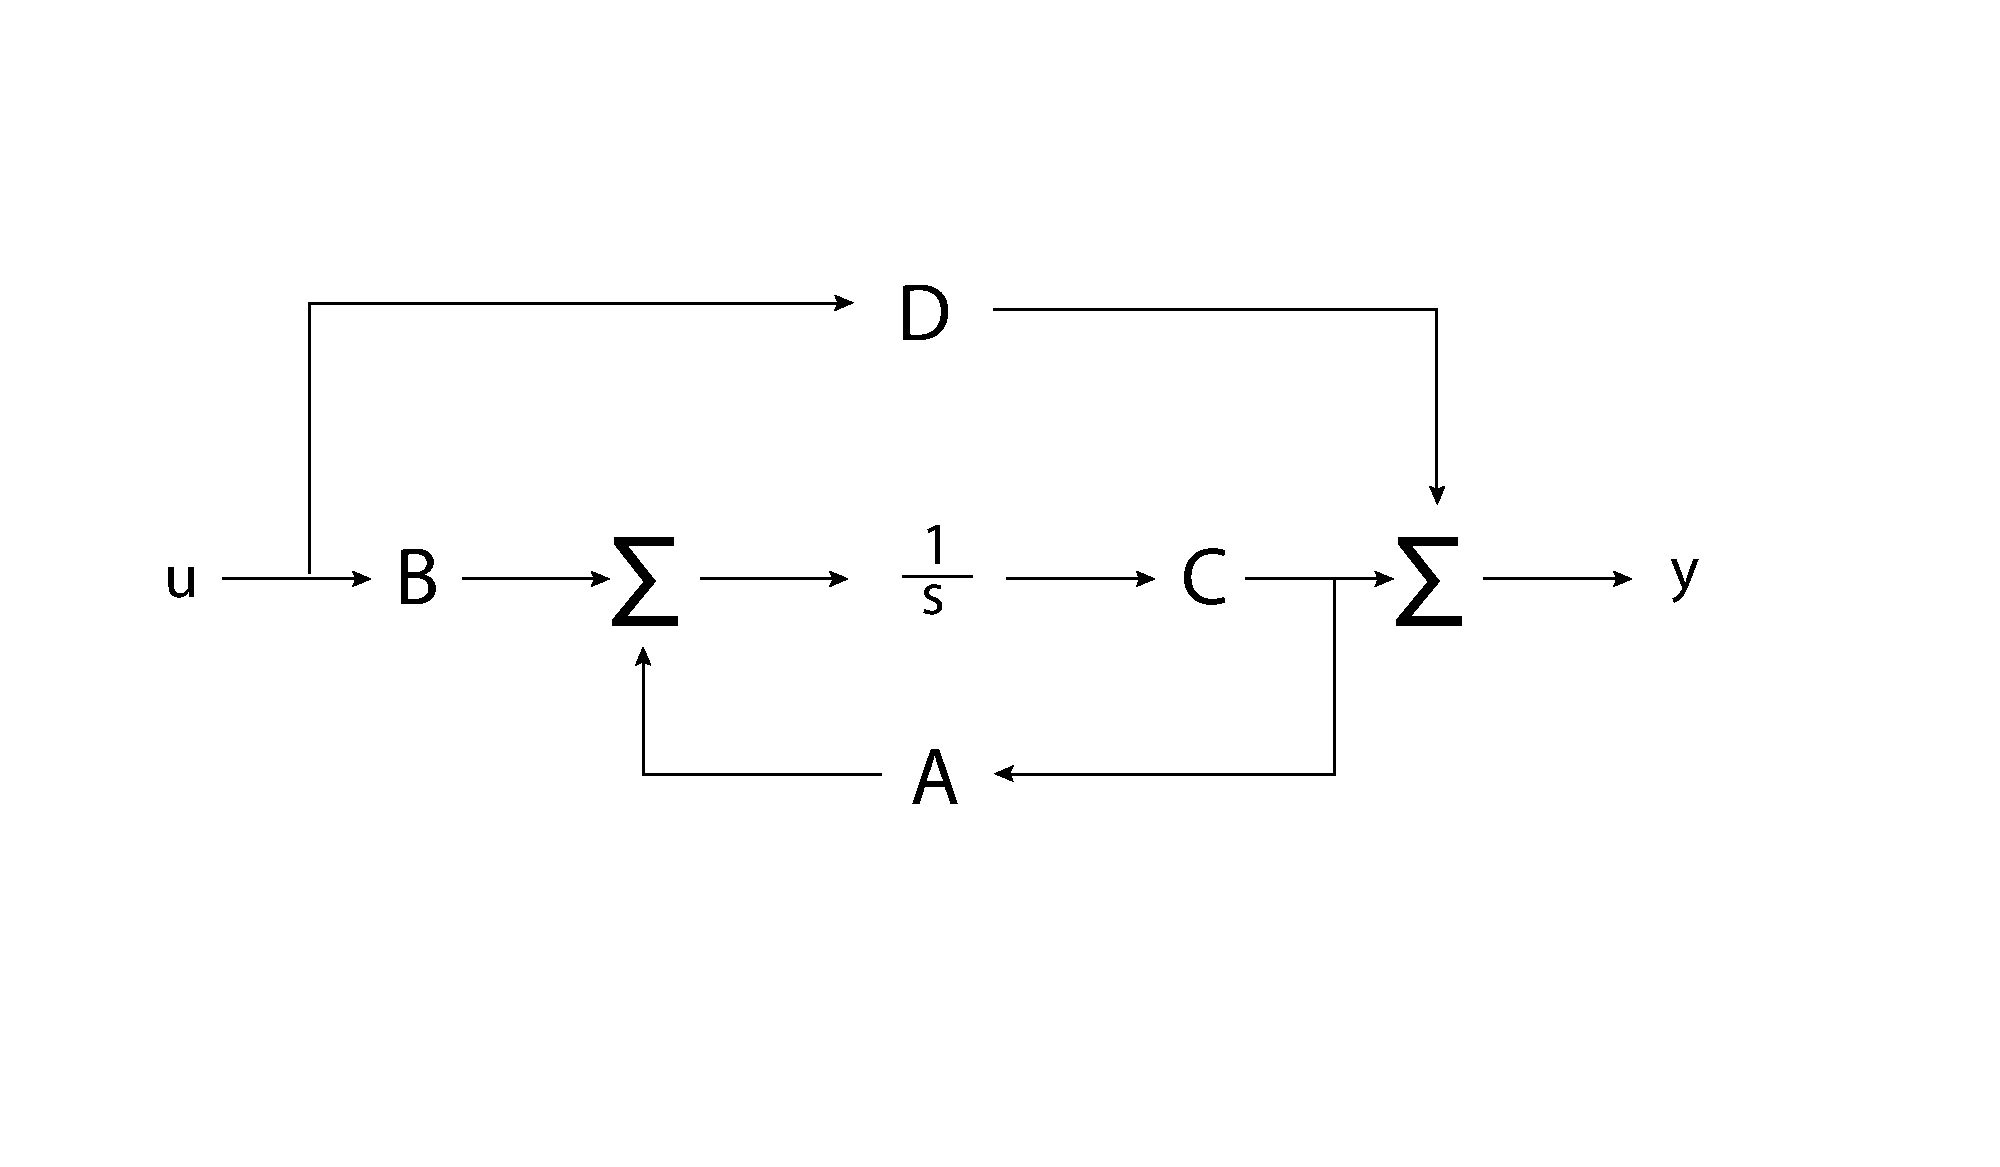
\includegraphics[width=0.8\textwidth]{images/statespace.pdf}
\caption{Représentation en bloque de l'espace d'état}
\end{figure}


... La modélisation des équations dans l'espace d'état suivra.

\subsubsection{Modélisation de l'algorithme génétique}

La méthodologie pour la modélisation de l'algorighme génétique de maximisation de la puissance de l'éolienne n'est pas encore fait et viendra.

\subsubsection{Modélisation du système de contrôle}

La méthodologie pour la modélisation du système de contrôle de l'éolienne n'est pas encore fait et viendra.

% subsection Analyse du modèle (end)
\subsection{Intégration du modèle} % (fold)
\label{sub:Intégration du modèle}

Le modèle après analyse doit être intégré à l'intérieur de la carte électronique de calcul (figure \ref{fig:carte}) conçu à cette fin. C'est une carte composée d'un microcontrôlleur 16 bit de 70 mips ayant 512 KB d'espace programme et 50 KB de mémoire vive

\begin{figure}[H]
\label{fig:carte}
\centering
\begin{tabular}{cc}
\includegraphics[width=0.4\textwidth]{images/carte-electronique-dessus.jpg} &
\includegraphics[width=0.4\textwidth]{images/carte-electronique-dessous.jpg}
\end{tabular}
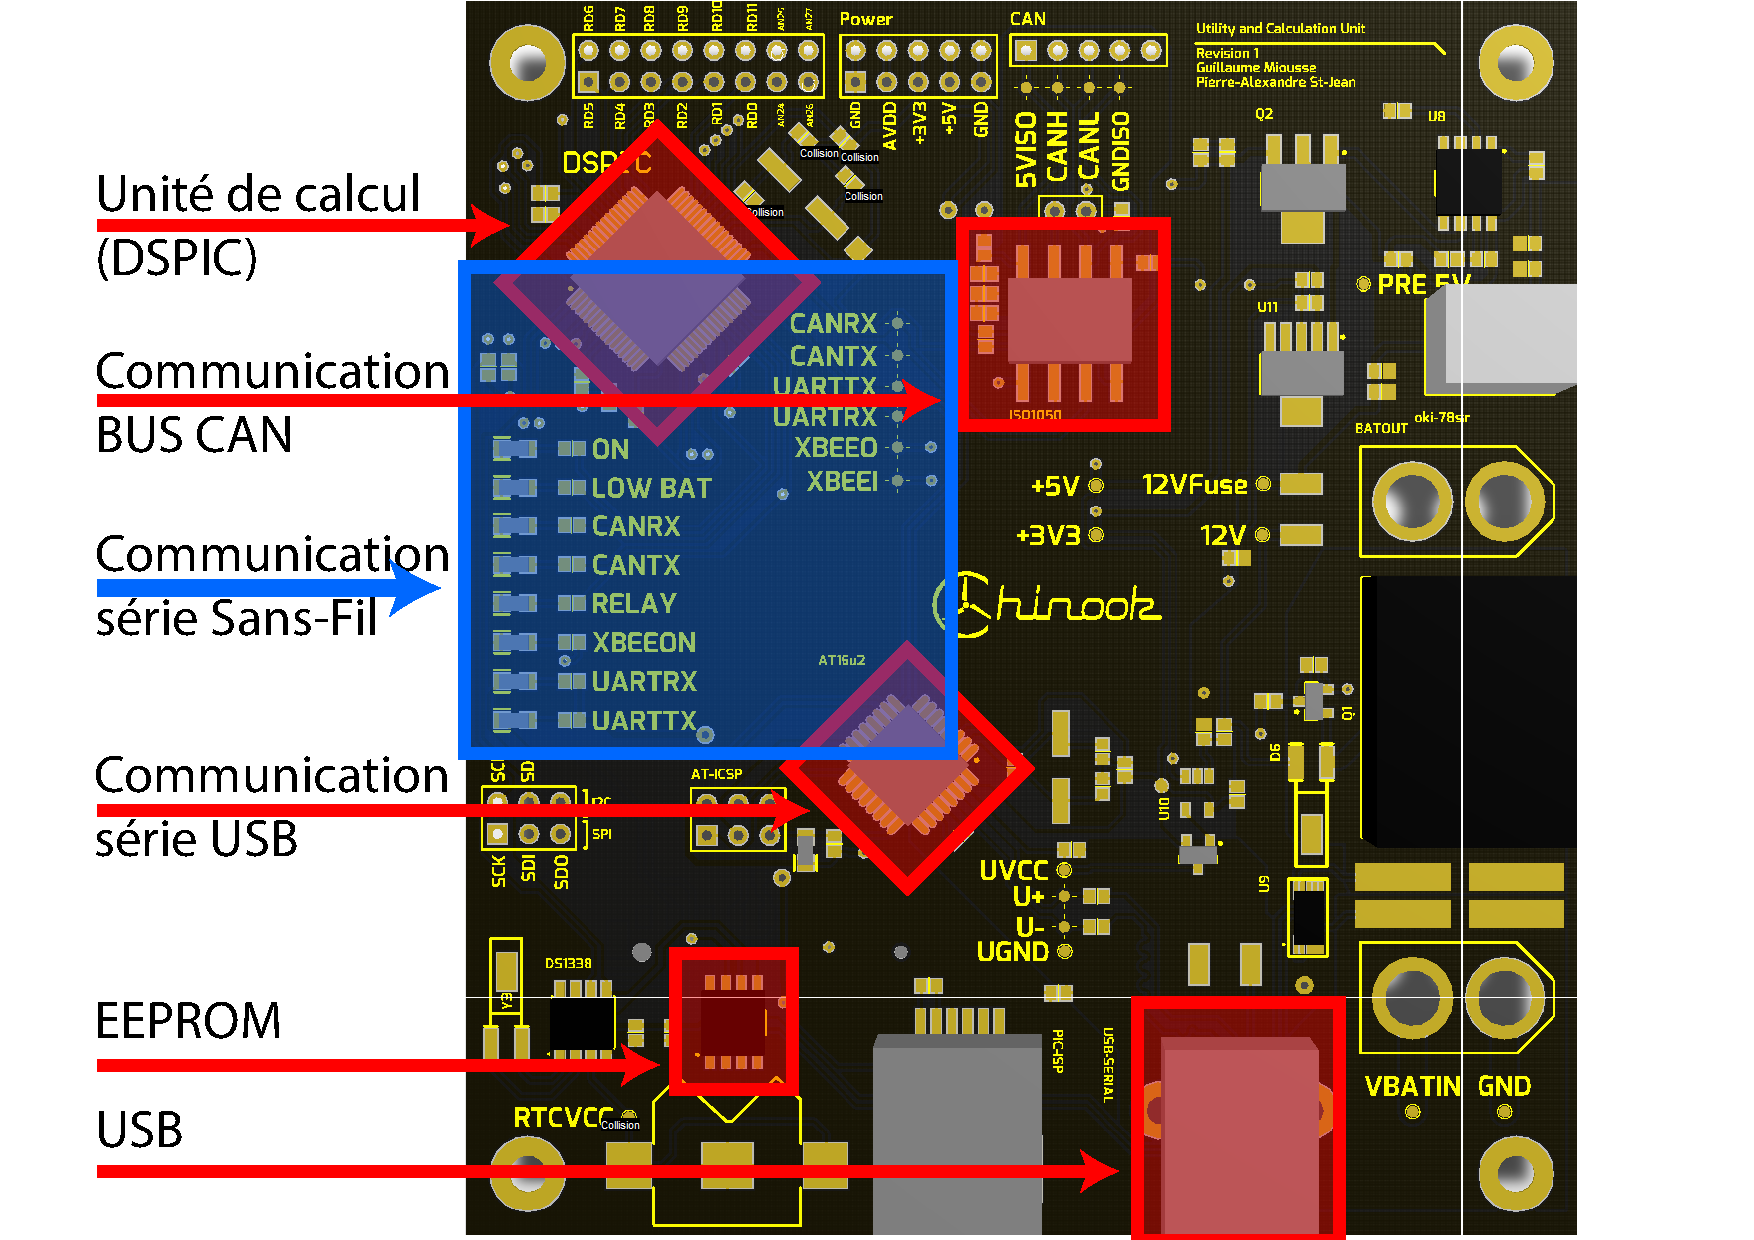
\includegraphics[width=0.6\textwidth]{images/carte-electronique-annote.pdf}
\caption{La carte électronique de calcul}
\end{figure}

Le code de contrôle doit y être intégré. Premièrement les bibliothèques de communication et l'application qui petmet de faire fonctionner la carte doit fonctionner. Puis on intègre le modèle mathématique en le transformant en programme en C utilisant les données reçus des autres cartes.

% subsection Intégration du modèle (end)
\subsection{Gestion du projet} % (fold)
\label{sub:Gestion du projet}



% subsection Gestion du projet (end)
% section Méthodologie (end)
